\documentclass{article}
\usepackage[utf8]{inputenc}
\usepackage{graphicx}
\usepackage{amsmath}

\title{Lecture 13}
\author{Scribed by: Erik Rosenstrom, Maharshi Parekh }
\date{October 7, 2019}



\begin{document}

\newtheorem{definition}{Definition}
\maketitle


\section{Planar Graphs}
\textbf{Recall:}

\begin{definition}{Euler Invariant: } 
$$|V_G| - |E_G| + |F_G| = 1 + |C_G|$$

\end{definition}
\begin{definition}{Outerplanar: }
A graph G is outerplanar if all vertices can be embedded on the outer face of the graph
\end{definition}

\subsection{Maximal Planar Graphs}
\begin{definition}{Maximal: }
A planar graph G is maximal if no more edges can be added while keeping it planar
\end{definition}


\textbf{Question:} If G is planar and maximal with n vertices, how many edges does G have?

When approaching a question like this it is helpful to come up with a small example to discover patterns. Let's start with n = 5

\begin{figure}[h!]
\centering
\includegraphics[width=0.6\textwidth]{"gt 1"}
\caption{Maximal Planar Graph, n = 5}
\end{figure}


\textbf{Lemma 1: }If G is maximal and planar, then every face is a triangle,$\ {K_3}$\\
\textbf{Proof:} Suppose for contradiction that some face has greater than or equal to 4 vertices. Among these 4 every edge must be in G. Otherwise, we could add one by cutting though the face. So, the embedding contains and embedding of$\ {K_4}$\ with all vertices on one face. This is a contradiction because$\ {K_4}$\ is not outer planar.\\

\textbf{Fact: } Every finite planar graph has a vertex degree at most 5.\\
\textbf{Proof: }We know that the maximum number of edges in a planar graph is$\ {3n-6}$. and the sum of degrees of all vertices is equal to twice the number of edges in the graph - \\ $$\sum_{v \in V} deg(v) = 2|E|$$ \\ Substituting in the value of maximum number of edges possible, we get: $$\sum_{v \in V} deg(v) = 2|E| \leq 6n-12 $$ \\
Taking the average for all vertices, we see that 
$$\frac{1}{n}(\sum_{v \in V} deg(v)) \leq 6 - \frac{12}{n} $$ \\
which is clearly less than 5. Hence, proved.

\vspace{5mm}

\textbf{Lemma 2: }If ${G}$ is 2-connected and ${\underline{G}}$ is an embedding of ${G}$, then every face of the embedding ${\underline{G}}$ is a cycle of G.

\textbf{Proof: } Suppose ${G}$ has a face that's not a cycle. Then some vertex on the face is visited more than once.
\newline Let us consider graph ${G'}$ where ${ \{ G' = G \backslash u\} }$
\begin{center}
    $$|V'| = |V| - 1$$
    $$|E'| = |E| - deg(u)$$
    $$|F'| = |F| - deg^{\star}(u) + 1$$ 
\end{center}
where ${deg^{\star}(u)}$ is the number of faces touching ${u}$ 
\newline Since the graph is 2-connected, we can use the Euler invariant $$|V_G| - |E_G| + |F_G| = 1 + |C_G|$$ for both ${G}$ and ${G'}$ as follows:\\
\begin{center}
    $$|V_G| - |E_G| + |F_G| = |V_G'| - |E_G'| + |F_G'|$$
    $$|V_G| - |E_G| + |F_G| = (|V_G| - 1) - (|E_G| - deg(u)) + (|F_G| - deg^{\star}(u)+1)$$
    $$deg(u) = deg^{\star}(u)$$
\end{center}
which is a contradiction. Hence, we can say that every face of the embedding is a cycle of the graph ${G}$.

\begin{definition}{Non-separating: }
A subgraph $H \subseteq G$ is non-separating if G and $G \backslash H$ are connected.
\end{definition}

\textbf{Theorem 1: }
If $G = (V,E) $ is planar and 3-connected then the faces of an embedding of ${G}$ are the non-separating induced cycles of ${G}$.\\
\textbf{Proof: }
Because ${G}$ is 3-connected, it is also 2-connected and therefore the faces are simple cycles. \\
Suppose ${C}$ is a non-separating induced cycle. Then, in any embedding ${C}$ maps to a Jordan curve, so, in order to be non-separating all other vertices must be inside of outside of the the embedding of ${C}$. In either case, this implies ${C}$ is a face. \\
Suppose ${C}$ is a face. It is an induced cycle because any other edges between vertices in ${C}$ would give a 2-vertex separator, contradicting the assumption that ${G}$ is 3-connected.\\
If ${C}$ separates ${G}$ then there are vertices ${u,v}$ such that every path from ${u}$ to ${v}$ contains a vertex of ${C}$.\\
By Menger's Theorem, there are 3 disjoint paths from ${u}$ to ${v}$.

\begin{figure}[h!]
\centering
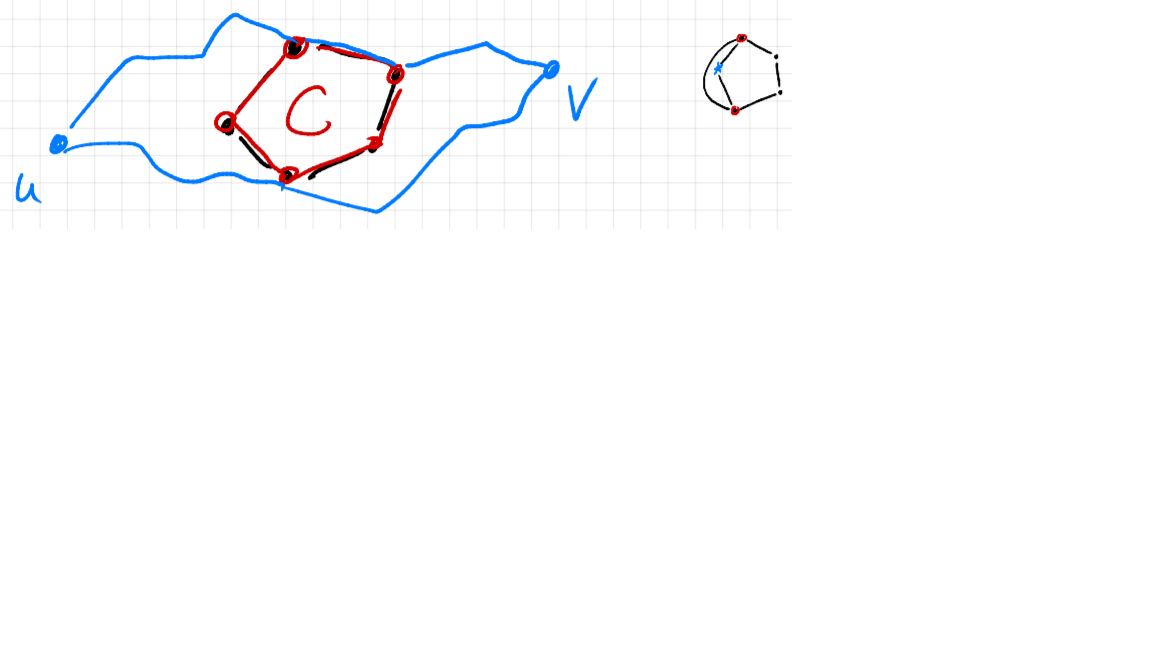
\includegraphics[width=0.6\textwidth]{gt2.png}
\caption{Application of Menger's Theorem}
\end{figure}

Two of these paths form a Jordan curve containing ${C}$. Note that there is no way to have another disjoint path that intersects ${C}$. Therefore, either ${C}$ could not be a face or G is not 3-connected. The contradiction implies the theorem. \\
\\
\textbf{Corollary: } Let ${G}$ be a planar, 3-connected graph. Then the faces of any two embeddings or ${G}$ are the same. 




\end{document}
